\chapter{Application: Erd\H{o}s' Pentagon Conjecture}

In 1983 \cite{erdosProblemsGraphTheory1984} Erd\H{o}s conjectured the following:

\begin{knownconjecture}
    The number of pentagons (5-cycles) in a triangle free graph $G$ is at most
    $\left(\frac{|G|}{5}\right)^5$.
\end{knownconjecture}

This conjecture remained open until 2012 when Grzesik
\cite{grzesikMaximumNumberFivecycles2012} eventually proved it to be true. Importantly
for us this paper used the classic flag algebras in a very direct and neat way.

\section{The Bounded Degree Conjecture}

Inspired by Erd\H{o}s' conjecture and looking for an application of our new framework we ask
the following question: Can we bound the number of pentagons in a triangle free graph
as a function of the maximum degree $\Delta(G)$?\footnote{Originally asked by E. Hurley}.
This leads us to the following \textit{bounded degree pentagon conjecture}:

\begin{conjecture}
    \label{conj:bounded_pentagon}
    The number of pentagons (5-cycles) in a triangle free graph $G$ is at asymptotically
    at most $\frac{|G|}{5}\left(\frac{\Delta(G)}{2}\right)^4=\frac{|G|}{5}\frac{\Delta(G)}{16}$.
\end{conjecture}

In this chapter we will show that if this conjecture is true it is tight, and show how we
used the semidefinite method on local flags to get an upper bound within a $\frac{1}{2}$
factor, showing an asymptotic upper bound of $\frac{|G|}{5}\frac{\Delta(G)}{8}$.

\begin{lemma}
    If the bounded degree pentagon conjecture is true then it is tight.
\end{lemma}

\begin{proof}
    Let $k\in\N$ even be given and take $G$ to be the $k/2$-blowup of $C_5$
    (figure \ref{fig:5_partite_graph}) meaning take 5 independent sets of size $k/2$ as
    "supernodes" then densely connect the supernodes into a 5-cycle.
    \begin{figure}[ht]
        \centering
        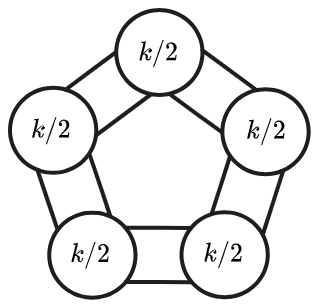
\includegraphics[scale=0.3]{5_partite_graph}
        \caption{Complete 5-partite graph on $5k/2$ vertices}
        \label{fig:5_partite_graph}
    \end{figure}
    This graph is triangle free: Notice that the induced subgraph on any 3 nodes is bipartite.
    Then we see that choosing
    a vertex from each of the 5 supernodes gives a distinct 5-cycle so there are at
    least $\left(\frac{k}{2}\right)^5$ pentagons in the graph (this is actually exact). But
    $|G|=\frac{5k}{2}$ and $\Delta(G)=k$ so we can rewrite this as
    $\left(\frac{k}{2}\right)^5 = \frac{|G|}{5}\left(\frac{\Delta(G)}{2}\right)^4$ meeting
    the bound. We can do this for any even $k=\Delta(G)$ so this holds asymptotically.
\end{proof}

We claim then the following theorem:
\begin{theorem}
    The number of pentagons in a triangle free graph is
    $\lesssim \frac{|G|}{5}\frac{\Delta(G)}{8}$
    as $\Delta(G) \to \infty$.
\end{theorem}

The rest of this chapter will show how we proved this. First we note the
following lemma:

\begin{lemma}
    It suffices to show the number of pentagons in a triangle free graph
    $G$ is bounded by $\frac{|G|}{5}\frac{\Delta(G)}{8}$ for regular $G$ only.
\end{lemma}

\begin{proof}
    Let $P(G)$ denote the number of pentagons in a graph $G$.
    Assume the lemma does not hold, i.e. assume that the bound holds for regular graphs but there
    exists $G$ with arbitrarily high $\Delta(G)$ which is non-regular such that the number
    of pentagons is strictly $P(G) > \frac{|G|}{5}\frac{\Delta(G)}{8}$.

    Let $G_0$ be such a triangle free non-regular graph. Construct a sequence $(G_i)_{i\in\N}$ as
    follows: To construct $G_{i+1}$ take two copies of $G_i$ then for each vertex $v\in V(G_i)$
    with $\deg v < \Delta(G_i)$ add an edge to $G_{i+1}$ between the two copies of $v$.

    We show by induction that each $G_i$ is triangle free, $\Delta(G_i)=\Delta(G_0)\ \forall i\in\N$
    and $P(G_i) > \frac{|G_i|}{5}\frac{\Delta(G)}{8}$. $G_0$ satisfies these conditions
    by assumption; Assume they hold for $G_i$. First we argue that $G_{i+1}$ has no
    triangles. Clearly each copy of $G_i$ has no triangles so we need to show the
    addition of edges between two 2 copies of $G_i$. Each edge we add is between
    two copies of a vertex $v\in V(G_i)$. This means
    each vertex in $G_{i+1}$ has at most 1 neighbour outside of its own copy of $G_i$.
    This means adding an edge between two copies of some $v$ cannot induce a cycle
    as the neighbourhoods of each copy of $v$ will be disjoint. Therefore $G_{i+1}$ is
    triangle free. Next we show $\Delta(G_{i+1})=\Delta(G_i)=\Delta(G_0)$; This is
    clear as we add edges only to vertices $v$ which have $\deg v < \Delta(G_i)=\Delta(G_0)$
    meaning we do not increase the maximum degree.
    Finally we show that $P(G_{i+1}) > \frac{|G_{i+1}|}{5}\frac{\Delta(G)}{8}$;
    This is also easy as $|G_{i+1}|=2|G_i|$ but $P(G_{i+1}) \geq 2 P(G_i)$ as we take
    two copies of $G_i$.

    Finally we note that the minimum degree increases by 1 every iteration if the
    graph is non-regular: $\delta(G_i) < \Delta(G_i) \implies \delta(G_{i+1})=\delta(G_i) + 1$.
    Then as $\Delta(G_i)=\Delta(G_0)\forall i\in\N$ this means there can be at most
    $\Delta(G_0)-\delta(G_0) \leq \Delta(G_0)$ iterations until we arrive at a regular
    $G_k$ which has the following properties: It is triangle free, $\Delta(G_k)=\Delta(G_0)$
    $P(G_k) > \frac{|G_k|}{5}\frac{\Delta(G_k)}{8}$.

    We could do this for any $G_0$ which contradicts our asymptotic bound on the
    class of triangle free regular graphs.
\end{proof}
